\باب{یکساں حال، برقرار چالو معاصر مشین}
جیسا کہ نام سے واضح ہے یہ وہ گھومنے والی مشین ہے جو ایک ہی رفتار سے گھومتی ہے اور یہ رفتار اس کو دیئے گئے برقی دباؤ کے تعدد پر منحصر ہوتی ہے۔

جب کسی جنریٹر پر بوجھ تبدیل کیا جائے یا اسے فراہم میکانی طاقت فراہم کرنے والے کی رفتار تبدیل کی جائے تو جنریٹر نئی صورتِ حال کے  مطابق چند ہی لمحات میں دوبارہ برقرار  صورت اختیار کر لیتا ہے۔اس برقرار چالو صورت میں اس کی رفتار، برقی دباؤ، برقی رو، درجہ حرارت وغیرہ  مقررہ رہتے ہیں۔اسی طرح اگر موٹر پر بوجھ تبدیل ہو تو اسے درکار طاقت اور برقی رو تبدیل ہوں گے۔بوجھ تبدیل ہونے سے پہلے موٹر برقرار مقررہ برقی رو حاصل کرتا رہتا ہے اور اس کا درجہ حرارت ایک مقررہ قیمت پر رہتا ہے۔اسی طرح بوجھ تبدیل ہونے کے چند ہی لمحات میں یہ دوبارہ ایک نئی برقرار چالو صورت اختیار کر لیتا ہے جہاں اس کی برقی رو ایک نئی قیمت پر برقرار رہتی ہے اور اس کا درجہ حرارت بھی ایک نئی قیمت اختیار کر لیتا ہے۔دو مختلف برقرار چالو، یکساں صورتوں کے درمیان چند لمحات کے لئے مشین عارضی صورت\فرہنگ{عارضی صورت}\حاشیہب{transient state}\فرہنگ{transient state} میں ہوتا ہے۔اس باب میں یکساں حال، برقرار چالو\فرہنگ{برقرار چالو}\حاشیہب{steady state}\فرہنگ{steady state} مشین پر تبصرہ کیا جائے گا۔ 

معاصر آلوں میں عموماً قوی لچھا ساکن رہتا ہے جبکہ میدانی لچھا معاصر رفتار سے گھومتا ہے۔قوی لچھوں کی برقی رو میدانی لچھوں کی برقی رو کی نسبت بہت زیادہ ہوتی ہے اور اسے سرک چھلوں کے ذریعہ گزارنا نہایت مشکل ہوتا ہے لہٰذا قوی لچھوں کو ساکن رکھا جاتا ہے جبکہ میدانی لچھوں کو گھمایا جاتا ہے۔

 ہم یہ دیکھ چکے ہیں کہ تین مرحلہ  لپٹے ساکن لچھوں میں اگر متوازن تین مرحلہ برقی رو ہو تو یہ ایک گھومتے مقناطیسی دباؤ کی موج کو جنم دیتی ہے۔اس گھومتے موج کی رفتار کو \اصطلاح{معاصر رفتار}\فرہنگ{معاصر رفتار}\حاشیہب{synchronous speed}\فرہنگ{synchronous speed}  کہتے ہیں۔ معاصر مشین کا گھومتا حصہ اسی رفتار سے گھومتا ہے۔ 

معاصر مشین کے میدانی لچھے کو یک سمتی برقی رو درکار ہوتی ہے جو یا تو سرک چھلوں کے ذریعہ اس تک باہر سے پہنچائی جاتی ہے یا پھر مشین کے دھرے پر ہی نسب ایک چھوٹی یک سمتی جنریٹر سے اسے فراہم کی جاتی ہے۔

میدانی لچھا ایک میدانی مقناطیسی دباؤ کو جنم دیتی ہے جو اس لچھے کے ساتھ ساتھ معاصر رفتار سے گھومتی ہے۔ لہٰذا معاصر مشین کے گھومتے اور ساکن لچھوں کے مقناطیسی دباؤ معاصر رفتار سے ہی گھومتے ہیں۔ اسی وجہ سے انہیں معاصر مشین کہتے ہیں۔

\حصہ{متعدد مرحلہ معاصر مشین}
معاصر مشین عموماً تین مرحلہ ہوتے ہیں۔ان کے تین مرحلہ ساکن قوی لچھے خلاء میں  \عددیء{120\degree} برقی زاویہ پر نسب ہوتے ہیں جبکہ اس کے میدانی لچھے گھومتے حصے پر نسب ہوتے ہیں اور ان میں یک سمتی برقی رو ہوتی ہے۔ 

اگر مشین کے گھومتے حصے کو بیرونی میکانی طاقت سے گھمایا جائے تو یہ مشین ایک معاصر جنریٹر کے طور پر کام کرتی ہے اور اس کے تین مرحلہ ساکن قوی لچھوں میں تین مرحلہ برقی دباؤ پیدا ہوتی ہے جس کا برقی تعدد گھومنے کے رفتار پر منحصر ہوتا ہے۔ اس کے برعکس اگر مشین کے تین  مرحلہ ساکن قوی لچھوں کو تین مرحلہ برقی طاقت مہیا کیا جائے تو یہ ایک معاصر موٹر کے طور کام کرتی ہے جو معاصر رفتار سے گھومتی ہے۔مشین کی کُل برقی قوت کے چند فی صد  برابر برقی قوت اس کے میدان لچھے کو درکار ہوتی ہے۔ گھومتے لچھے تک برقی دباؤ مختلف طریقوں سے پہنچائی جاتی ہے۔شکل \حوالہ{شکل_معاصر_سرک_چھلے}  میں گھومتے لچھے تک موصل \اصطلاح{سرک چھلے}\فرہنگ{سرک چھلے}\حاشیہب{slip rings}\فرہنگ{slip rings}  کی مدد سے یک سمتی برقی رو پہنچانے کا طریقہ دکھایا گیا ہے۔ یہ سرک چھلے اُسی دھرے  پر نسب ہوتے ہیں جس پر گھومتا لچھا نسب ہوتا ہے اور یہ اس لچھے کے ساتھ یکساں طور پر گھومتے ہیں۔ سرک چھلوں  کے بیرونی سطح پر کاربن کے ساکن بُش، اسپرنگ  کی مدد سے ان کے ساتھ دبا کر رکھے جاتے ہیں۔ جب مشین چلتی ہے  کاربن کے بُش ان سرک چھلوں پر سرکتے ہیں۔ اسپرنگ کا دباؤ ان کا برقی جوڑ مضبوط رکھتا ہے اور ان کے مابین چنگاریاں نہیں نکلتی۔ کاربن بُش کے ساتھ برقی تار لگی ہے۔ اس طرح یک سمتی برقی رو \عددیء{I_r} ، کاربن بُش\فرہنگ{کاربن بش}\فرہنگ{بش}\حاشیہب{carbon bush}\فرہنگ{carbon bush} سے سرک چھلوں اور یہاں سے گھومتے لچھے تک پہنچتی ہے۔

بڑے معاصر مشین میں میدانی یک سمتی برقی رو عموماً ایک بدلتی رو برقی جنریٹر سے حاصل کی جاتی ہے جو معاصر مشین کے دھرے پر ہی نسب ہوتی ہے اور اس کے ساتھ یکساں طور پر گھومتی ہے۔اس چھوٹے جنریٹر کی برقی دباؤ کو دھرے پر ہی نسب الیکٹرانکس کی مدد سے یک سمتی برقی دباؤ میں تبدیل کیا جاتا ہے۔ یوں سرک چھلے کی ضرورت نہیں رہتی۔سرک چھلے رگڑ کی وجہ سے خراب ہوتے ہیں جس کی وجہ سے معاصر مشین کو مرمت کی خاطر بند کرنا پڑتا ہے جو بہت مہنگا پڑتا ہے۔
\begin{figure}
\centering
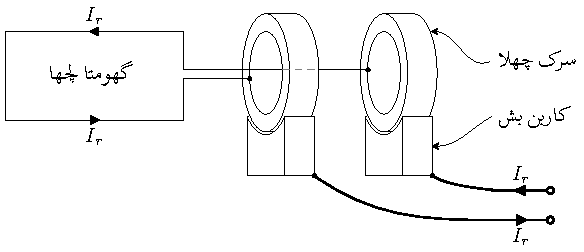
\includegraphics{figSynchronousSlipRings}
\caption{کاربن بُش اور سرک چھلوں سے لچھے تک برقی رو پہنچایا گیا ہے۔}
\label{شکل_معاصر_سرک_چھلے}
\end{figure}

اُبھرے قطب\فرہنگ{قطب!ابھرے}\حاشیہب{salient poles} مشین پانی سے چلنے والے سست رفتار جنریٹر اور  عام استعمال کے موٹروں کے لئے موزوں ہوتے ہیں جبکہ ہموار قطب\فرہنگ{قطب!ہموار}\حاشیہب{non-salient poles}\فرہنگ{non-salient poles} مشین تیز رفتار دو یا چار قطب والے ٹربائن جنریٹروں کے لئے موزوں ہوتے ہیں۔

کسی بھی مملکت کو درکار برقی توانائی ایک برقی جنریٹر سے دینا ممکن نہیں، لہٰذا حقیقت میں کچھ درجنوں سے لیکر کئی سو برقی جنریٹر بیک وقت یہ فریضہ سر انجام دے رہے ہوتے ہیں۔ ایک سے زیادہ جنریٹر استعمال کرنا فائدہ مند ثابت ہوتا ہے۔ اوّل تو برقی توانائی کی ضرورت کے مطابق جنریٹر چالو کئے جا سکتے ہیں اور پھر ان جنریٹروں کو ضرورت کی جگہ کے ممکنہ طور پر قریب نسب کیا جا سکتا ہے۔ کسی بھی اس طرح کے بڑے نظام میں ایک جنریٹر کی حیثیت بہت کم ہو جاتی ہے۔ ایک جنریٹر چالو یا بند کرنے سے پورے نظام پر کوئی خاص فرق نہیں پڑتا۔ اس صورت میں ہم اس نظام کو ایک مقررہ برقی دباؤ اور ایک مقررہ برقی تعدد رکھنے والا نظام تصور کر سکتے ہیں۔ معاصر جنریٹروں کے کئی اہم پہلو با آسانی سمجھے جا سکتے ہیں اگر یہ تصور کر لیا جائے کہ یہ ایک ایسے ہی نظام سے جوڑا گیا ہے۔

مساوات \حوالہ{مساوات_گھومتے_مشین_مروڑ_اور_بہاو}  ایک معاصر مشین کا قوت مروڑ بتلاتا ہے۔اس مساوات کے مطابق برقی مقناطیسی قوت مروڑ کی کوشش ہوتی ہے کہ وہ مشین میں موجود عمل کرنے والے مقناطیسی دباؤ کو سیدھ میں لائے۔ برقرار  چالو  مشین کا برقی مقناطیسی قوت مروڑ اور اس کے دھرے پر لاگو میکانی قوت مروڑ برابر ہوتے ہیں۔ جب مشین ایک جنریٹر کی حیثیت سے استعمال ہو تب میکانی طاقت  دھرے کو گھماتا ہے اور گھومتے لچھے کا مقناطیسی دباؤ کُل مقناطیسی دباؤ سے گھومنے کی سمت میں آگے ہوتا ہے۔ مساوات \حوالہ{مساوات_گھومتے_مشین_مروڑ_اور_بہاو} سے حاصل قوت مروڑ اس صورت میں گھومنے کو روکنے کی کوشش کرتا ہے۔میکانی طاقت چلتے پانی، ایندھن سے چلتے انجن وغیرہ سے حاصل ہو سکتا ہے۔ اسی طرح اگر مشین ایک موٹر کی حیثیت سے استعمال ہو رہا ہو، تب صورت اس کے بالکل اُلٹ ہو گی۔

اگر کُل مقناطیسی بہاو  \عددیء{\phi_{ar}} اور گھومتے لچھے کا مقناطیسی دباؤ \عددیء{\tau_r} تبدیل نہ ہو تب اسی مساوات کے مطابق مشین کا قوت مروڑ  \عددیء{\sin \theta_r} کے ساتھ تبدیل ہو گا۔ اگر زاویہ \عددیء{\theta_r} صفر ہو تب یہ قوت مروڑ بھی صفر ہو گا۔ اب  تصور کریں کہ یہی مشین ایک موٹر کے طور پر استعمال ہو رہی ہو۔ جیسے جیسے موٹر پر لدا میکانی بوجھ بڑھایا جائے ویسے ویسے اس کے دھرے پر میکانی قوت مروڑ بڑھے گی۔ موٹر کو برابر کا برقی مقناطیسی قوت مروڑ پیدا کرنا ہو گا جو یہ زاویہ بڑھا کر کرتا ہے۔یہاں یہ سمجھنا ضروری ہے کہ موٹر ہر وقت معاصر رفتار سے ہی گھومتا ہے اور وہ یہ زاویہ پل بھر کے لئے آہستہ ہو کر ضرورت کے مطابق درست کرتا ہے۔یعنی موٹر کا زاویہ \عددیء{\theta_r} ہر وقت میکانی قوت مروڑ کا تعقب\فرہنگ{تعقب}\حاشیہب{hunting}\فرہنگ{hunting}  کرتی ہے۔

اگر موٹر پر لدا میکانی بوجھ بتدریج بڑھایا جائے تو ایک لمحہ آئے گا جب زاویہ \عددیء{\theta_r} نوے درجہ یعنی  \عددیء{\tfrac{\pi}{2}} ریڈیئن تک پہنچ جائے گا۔ اس لمحہ موٹر اپنی انتہائی قوت مروڑ\فرہنگ{قوت مروڑ!انتہائی}\حاشیہب{pull out torque}\فرہنگ{torque!pull out}  پیدا کر رہی ہو گی۔ اگر بوجھ  مزید بڑھایا جائے تو موٹر کسی بھی صورت میں اس کے مقابلے کا قوت مروڑ نہیں پیدا کر سکتی اور یہ موٹر رکھ جائے گی۔ ہم کہتے ہیں کہ موٹر نے \اصطلاح{غیر معاصر}\فرہنگ{غیر معاصر}\حاشیہب{lost synchronism} صورت اختیار کر لی ہے۔ مساوات سے یہ ظاہر ہے کہ کُل مقناطیسی بہاو یا گھومتے لچھے کا مقناطیسی دباؤ بڑھا کر اس انتہائی قوت مروڑ کی مقدار بڑھائی جا سکتی ہے۔

یہی صورت اگر مشین برقی جنریٹر کے طور پر استعمال کی جائے سامنے آتی ہے۔ جب بھی مشین غیر معاصر صورت اختیار کرے اسے جلد خود کار  دور شکن\فرہنگ{دور شکن}\حاشیہب{circuit breaker}\فرہنگ{circuit breaker} کی مدد سے برقی بھم رسانی سے الگ کر دیا جاتا ہے۔

ہم نے دیکھا کہ ایک معاصر موٹر صرف اور صرف معاصر رفتار سے ہی گھوم سکتی ہے اور صرف اسی رفتار پر گھومتی صورت میں قوت مروڑ پیدا کر سکتی ہے لہٰذا اگر اسے ساکن حالت سے چالو  کرنے کی کوشش کی جائے تو یہ کوشش ناکام رہے گی۔ ایسے موٹر کو پہلے کسے اور طریقے سے معاصر رفتار تک لایا جاتا ہے اور پھر اسے چالو کیا جاتا ہے۔ ایسا عموماً ایک چھوٹی \اصطلاح{امالی موٹر}\حاشیہب{induction motor}  کی مدد سے کیا جاتا ہے جو بے بوجھ معاصر موٹر کو، اس کے معاصر رفتار تک لے آتا ہے اور پھر اس معاصر موٹر کو چالو کیا جاتا ہے۔ ایسی امالہ موٹر معاصر موٹر کے دھرے پر ہی نسب ہوتی ہے۔

\حصہ{معاصر مشین کے امالہ}
 ہم تصور کرتے ہیں کہ مشین دو قطب اور تین مرحلہ ہے اور اس کے لچھے ستارہ نما جڑے  ہیں۔اس طرح لچھوں میں برقی رو، تار برقی رو\حاشیہب{line current} ہی ہو گی اور ان پر لاگو برقی دباؤ، یک مرحلہ برقی دباؤ ہو گی۔ایسا کرنے سے مسئلہ پر غور کرنا آسان ہو جاتا ہے جبکہ نتیجہ کسی بھی موٹر کے لئے درست ہوتا ہے۔

شکل \حوالہ{شکل_معاصر_تین_دور_دو_قطب}  میں ایک ایسا تین مرحلہ دو قطب معاصر مشین دکھایا گیا ہے۔ اس کا گھومتا حصہ نلکی نما ہے۔اس کو دو قطب کا مشین یا پھر \عددیء{P} قطب کے مشین کا دو قطب کا حصہ سمجھا جا سکتا ہے۔

 یہاں گچھ لچھے دکھائے گئے ہیں لیکن حقیقت میں پھیلے لچھے ہی استعمال ہوتے ہیں اور انہیں درحقیقت پھیلے لچھے ہی سمجھا جائے۔ اس طرح ہر لچھا سائن نما برقی دباؤ پیدا کرتا ہے جس کی چوٹی لچھے کی مقناطیسی محور کی سمت میں ہوتی ہے۔  چونکہ معاصر مشین میں گھومتے لچھے میں یک سمتی رو ہی ہوتا ہے لہٰذا اس کا مقناطیسی دباؤ ہر لمحہ گھومتے حصے کی مقناطیسی محور کی سمت میں ہی رہتا ہے۔ یہ شکل میں دکھایا گیا ہے۔ اس طرح گھومتے لچھے کا مقناطیسی دباؤ گھومتے حصے کے ساتھ ساتھ معاصر رفتار سے گھومتا ہے۔

ہم فرض کرتے ہیں کہ مشین معاصر رفتار \عددیء{\omega} سے گھوم رہی ہے۔ اس طرح اگر لمحہ \عددیء{t=0} پر مرحلہ\حاشیہب{phase} \عددیء{a} اور گھومتے لچھے کے مقناطیسی محور ایک ہی سمت میں ہوں تب کسی بھی لمحہ \عددیء{ت} پر ان کے مابین زاویہ \عددیء{\theta=\omega t} ہو گا۔
\begin{figure}
\centering
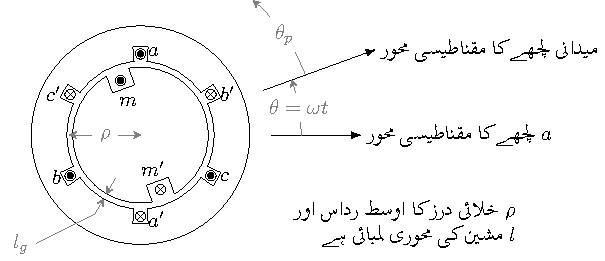
\includegraphics{figSynchronousThreePhaseTwoPole}
\caption{تین مرحلہ، دو قطب معاصر مشین۔}
\label{شکل_معاصر_تین_دور_دو_قطب}
\end{figure}
امالہ کے حساب لگانے کے لئے شکل \حوالہ{شکل_معاصر_تین_دور_دو_قطب}  سے رجوع کریں۔ شکل میں محیط پر خلائی درز یکساں ہے  اور اس کی رداسی سمت میں لمبائی \عددیء{l_g} ہے۔ساکن حصے میں شگافوں کے اثر کو نظرانداز کیا گیا ہے۔محور سے خلائی درز تک کا اوسط رداسی فاصلہ \عددیء{\rho} ہے اور مشین کی دھرے کی سمت میں محوری لمبائی \عددیء{l} ہے۔

کسی بھی لچھے کے خود امالہ کا حساب کرتے وقت باقی سب لچھوں کو نظرانداز کریں۔ اس کا مطلب ہے کہ آپ تصور کریں کہ باقی سب لچھوں میں برقی رو صفر ہے یعنی ان لچھوں  کے سرے آزاد رکھے گئے ہیں۔ حقیقت میں اگر آپ کبھی لچھوں کے خود امالہ کو مشین کی مدد سے ناپنا چاہیں تو آپ باقی سب لچھوں کے سرے آزاد ہی رکھیں گے۔ 

\جزوحصہ{خود امالہ}
گھومتے یا ساکن لچھے کی خود امالہ \عددیء{L} زاویہ \عددیء{\theta} پر منحصر نہیں۔ ان میں سے کسی بھی لچھے کی مقناطیسی دباؤ  \عددیء{\tau}
\begin{align}
\tau=k_w \frac{4}{\pi}\frac{N i}{2} \cos \theta_p
\end{align}
سے خلائی درز میں کثافت مقناطیسی بہاو \عددیء{B}  پیدا ہو گی جہاں	
\begin{align}
B=\mu_0 H=\mu_0 \frac{\tau}{l_g}=\mu_0 k_w \frac{4}{\pi}\frac{N i}{2 l_g} \cos \theta_p
\end{align}
یہ مساوات زاویہ \عددیء{\theta_p} کے ساتھ بدلتی کثافتِ مقناطیسی دباؤ \عددیء{B} بتلاتی ہے۔ اس لچھے کا ایک قطب پر  کُل مقناطیسی بہاو \عددیء{\phi} کا حساب کرنے کے لئے ہمیں اس مساوات کا سطحی تکمل\فرہنگ{سطحی تکمل}\حاشیہب{surface integral} یوں لینا ہو گا۔
\begin{gather}
\begin{aligned}\label{مساوات_معاصر_بہاو_بذریع_سطحی_تکمل}
\phi&=\int \kvec{B} \cdot \dif \kvec{S}\\
&=\int_{-\frac{\pi}{2}}^{+\frac{\pi}{2}} B l \rho \dif \theta_p\\
&=\mu_0 k_w \frac{4}{\pi}\frac{N i}{2 l_g} l \rho \int_{-\frac{\pi}{2}}^{+\frac{\pi}{2}}  \cos  \theta_p \dif \theta_p\\
&=\frac{4 \mu_0 k_w N i l \rho}{\pi l_g}
\end{aligned}
\end{gather}
اب ہم اس لچھے کی خود امالہ \عددیء{L} مساوات \حوالہ{مساوات_مقناطیسی_دور_خود_امالہ_تعریف} میں جزو پھیلاو \عددیء{k_w} کا اثر شامل کرتے ہوئے  حاصل کر سکتے ہیں۔
\begin{align}
L=\frac{\lambda}{i}=\frac{k_w N \phi}{i}=\frac{4 \mu_0 k_w^2 N^2  l \rho}{\pi l_g}
\end{align}
یہ مساوات اس شکل میں کسی بھی لچھے کی خود امالہ دیتا ہے۔یعنی
\begin{align}\label{مساوات_معاصر_تین_ساکن_امالہ_برابر}
L_{aa0}=L_{bb0}=L_{cc0}=\frac{4 \mu_0 k_{wa}^2 N_a^2  l \rho}{\pi l_g}
\end{align}
اور
\begin{align}
L_{mm0}=\frac{4 \mu_0 k_{wm}^2 N_m^2  l \rho}{\pi l_g}
\end{align}
\جزوحصہ{مشترکہ امالہ}
اب ہم دو لچھوں کا مشترکہ امالہ حاصل کرتے ہیں۔تصور کریں کہ صرف  گھومتا لچھا مقناطیسی بہاو پیدا کر رہا ہے۔ ہم اس کا وہ حصہ جو \عددیء{a} لچھے  سے گزرے کا حساب لگا کر ان کا مشترکہ امالہ حاصل کریں گے۔شکل \حوالہ{شکل_معاصر_تین_دور_دو_قطب}  میں گھومتے اور \عددیء{a} لچھے کے مابین کا زاویہ \عددیء{\theta} ہے۔اس صورت میں وہ مقناطیسی بہاو جو \عددیء{(-\tfrac{\pi}{2}-\theta)< \theta_p < (\tfrac{\pi}{2}-\theta)} کے مابین ہو، \عددیء{a} لچھے سے گزرے گا۔ اس مقناطیسی بہاو کا حساب مساوات \حوالہ{مساوات_معاصر_بہاو_بذریع_سطحی_تکمل}  میں تکمل کے حدود تبدیل کر کے یوں حاصل ہو گا۔
\begin{gather}
\begin{aligned}
\phi_{am}&=\int \kvec{B} \cdot \dif \kvec{S}\\
&=\int_{-\frac{\pi}{2}-\theta}^{+\frac{\pi}{2}-\theta} B l \rho \dif \theta_p\\
&=\mu_0 k_{wm} \frac{4}{\pi}\frac{N_m i_m}{2 l_g} l \rho \int_{-\frac{\pi}{2}-\theta}^{+\frac{\pi}{2}-\theta} \cos \theta_p \dif \theta_p\\
&=\frac{4 \mu_0 k_{wm}  N_m i_m l \rho}{\pi l_g} \cos \theta
\end{aligned}
\end{gather}
اس مساوات سے ان کا مشترکہ امالہ  یہ ہے 
\begin{align}
L_{am}=\frac{\lambda_{am}}{i_m}=\frac{k_{wa} N_a \phi_{am}}{i_m}=\frac{4 \mu_0 k_{wa} k_{wm} N_a N_m l \rho}{\pi l_g} \cos \theta
\end{align}
اس کو یوں لکھ سکتے ہیں
\begin{align}\label{مساوات_معاصر_ساکن_گھومتا_مشترکہ_امالہ}
L_{am}=L_{am0} \cos \theta
\end{align}
جہاں جیسے پہلے ذکر ہوا زاویہ \عددیء{\theta} گھومنے کی رفتار پر منحصر ہے یعنی  \عددیء{\theta=\omega t} اور \عددیء{L_{am0}}  یہ ہے
\begin{align}
L_{am0}=\frac{4 \mu_0 k_{wa} k_{wm} N_a N_m l \rho}{\pi l_g} 
\end{align}
اگرچہ یہ مساوات ایک گھومتے اور ایک ساکن لچھے کے لئے نکالا گیا ہے درحقیقت یہ اس شکل میں کسی بھی دو لچھوں کے لئے درست ہے۔ یہ دونوں لچھے ساکن ہوتے تب بھی جواب یہی آتا۔ اگر یہ دونوں گھومتے ہوتے تب بھی جواب یہی آتا۔ لہٰذا دو ساکن  یکساں لچھے مثلاً \عددیء{a} اور \عددیء{b} جن کے مابین \عددیء{120\degree} کا زاویہ ہے کا آپس کا مشترکہ امالہ یہ ہو گا
\begin{align}
L_{ab}&=\frac{4 \mu_0 k_{wa} k_{wb} N_a N_b l \rho}{\pi l_g} \cos 120\degree=-\frac{2 \mu_0 k_{wa}^2  N_a^2 l \rho}{\pi l_g}
\end{align}
جہاں دونوں لچھے بالکل یکساں ہونے کی بدولت  \عددیء{k_{wb}=k_{wa}} اور \عددیء{N_b=N_a} لئے گئے ہیں۔اگر تینوں ساکن لچھے بالکل یکساں ہو تب ہم اس مساوات اور مساوات \حوالہ{مساوات_معاصر_تین_ساکن_امالہ_برابر} کی مدد سے یہ لکھ سکتے ہیں۔ 
\begin{align}\label{مساوات_معاصر_ساکن_مشترکہ_امالہ}
L_{ab}=L_{bc}=L_{ca}=-\frac{L_{aa0}}{2}
\end{align}
%
\جزوحصہ{معاصر امالہ}
مشین پر لاگو برقی دباؤ کو مشین کے لچھوں کی خود امالہ، مشترکہ امالہ اور لچھوں میں برقی رو کی مدد سے لکھا جا سکتا ہے۔ یہ کرنے کے لئے ہم پہلے  لچھوں کی ارتباط بہاو \عددیء{\lambda} کو ان کے امالہ اور ان میں برقی رو کی مدد سے یوں لکھتے ہیں۔
\begin{gather}
\begin{aligned}
\lambda_a&=L_{aa} i_a+L_{ab} i_b +L_{ac} i_c+L_{am} I_m\\
\lambda_b&=L_{ba} i_a+L_{bb} i_b +L_{bc} i_c+L_{bm} I_m\\
\lambda_c&=L_{ca} i_a+L_{cb} i_b +L_{cc} i_c+L_{cm} I_m\\
\lambda_m&=L_{ma} i_a+L_{mb} i_b +L_{mc} i_c+L_{mm} I_m
\end{aligned}
\end{gather}
ان مساوات میں ساکن لچھوں کے بدلتی برقی رو  کو چھوٹے حروف یعنی \عددیء{i_a,i_b,i_c} سے ظاہر کیا گیا ہے جبکہ گھومتے میدانی لچھے کے یک سمتی برقی رو کو بڑے حرف  \عددیء{I_m} سے ظاہر کیا گیا ہے۔

ان چار مساوات میں سے ہم کسی ایک کو چُنتے ہیں اور اسے حل کرتے ہیں۔ چونکہ یہ چاروں مساوات ایک طرح کے ہیں اس لئے باقی بھی ایسے ہی حل ہوں گے۔ ہم ان میں سے پہلے مساوات لیتے ہیں یعنی
\begin{align}\label{مساوات_معاصر_ارتباط_الف_کل}
\lambda_a&=L_{aa} i_a+L_{ab} i_b +L_{ac} i_c+L_{am} I_m
\end{align}
 مساوات \حوالہ{مساوات_معاصر_تین_ساکن_امالہ_برابر}  ہمیں  \عددیء{a} لچھے کا خود امالہ دیتا ہے۔ یہ مساوات یہ تصور کر کے نکالا گیا تھا کہ اس لچھے کا پورا مقناطیسی بہاو خلائی درز سے گزرتا ہے۔ حقیقت میں ایسا نہیں ہوتا اور کچھ مقناطیسی بہاو اس خلائی درز میں سے گزر کر دوسری جانب نہیں پہنچتا۔ ایسے مقناطیسی بہاو کی وجہ سے رستا امالہ \عددیء{L_{al}}  وجود میں آتا ہے۔ یہ بالکل ٹرانسفارمر کے رستا امالہ کی طرح ہے۔ یوں اس لچھے کا کُل خود امالہ \عددیء{L_{aa}}  یہ ہے۔
\begin{align}\label{مساوات_معاصر_الف_خود_کل_امالہ}
L_{aa}=L_{aa0}+L_{al}
\end{align}
ہم مساوات \حوالہ{مساوات_معاصر_تین_ساکن_امالہ_برابر}،  مساوات \حوالہ{مساوات_معاصر_ساکن_گھومتا_مشترکہ_امالہ}،  مساوات \حوالہ{مساوات_معاصر_ساکن_مشترکہ_امالہ}  اور مساوات \حوالہ{مساوات_معاصر_الف_خود_کل_امالہ}  کی مدد سے مساوات \حوالہ{مساوات_معاصر_ارتباط_الف_کل}  کو یوں لکھتے ہیں۔
\begin{gather}
\begin{aligned}\label{مساوات_معاصر_ارتباط_الف}
\lambda_a&=\left(L_{aa0}+L_{al} \right)i_a-\frac{L_{aa0}}{2} i_b -\frac{L_{aa0}}{2} i_c+L_{am0} I_m \cos \omega t \\
&=\left(L_{aa0}+L_{al} \right)i_a-\frac{L_{aa0}}{2} \left( i_b+i_c \right)+L_{am0} I_m \cos \omega t
\end{aligned}
\end{gather}
اب تین مرحلہ برقی رو مجموعہ صفر ہوتا ہے یعنی 
\begin{align}
i_a+i_b+i_c=0
\end{align}
لہٰذا مساوات \حوالہ{مساوات_معاصر_ارتباط_الف}  میں اس کو استعمال کرتے ملتا ہے
\begin{gather}
\begin{aligned}
\lambda_a&=\left(L_{aa0}+L_{al} \right)i_a-\frac{L_{aa0}}{2} \left( -i_a \right)+L_{am0} I_m \cos \omega t\\
&=\left(\frac{3}{2} L_{aa0}+L_{al} \right)i_a+L_{am0} I_m \cos \omega t\\
&=L_s i_a+L_{am0} I_m \cos \omega t
\end{aligned}
\end{gather}
جہاں
\begin{align}\label{مساوات_معاصر_معاصر_امالہ}
L_s=\frac{3}{2} L_{aa0}+L_{al}
\end{align}
کو \اصطلاح{معاصر امالہ}\فرہنگ{معاصر امالہ}\حاشیہب{synchronous inductance}\فرہنگ{synchronous inductance} کہتے ہیں۔

اس مساوات اور مساوات \حوالہ{مساوات_تبادلہ_گھومتا_موج}  پر ایک مرتبہ دوبارہ غور کریں۔ یہ دونوں ملتے جلتے ہیں۔ وہاں کُل گھومتا مقناطیسی دباؤ ایک لچھے کی مقناطیسی دباؤ کے \عددیء{\tfrac{3}{2}}  گھنّا تھا اور یہاں معاصر امالہ ایک لچھے کی امالہ کے \عددیء{\tfrac{3}{2}} گھنّا ہے۔ یہ دو مساوات درحقیقت ایک ہی حقیقت کے دو پہلو ہیں۔

معاصر امالہ تین حصوں پر مشتمل ہے۔ پہلا حصہ \عددیء{L_{aa0}} ہے جو \عددیء{a} لچھے کا خود امالہ ہے۔ دوسرا حصہ \عددیء{\tfrac{L_{aa0}}{2}}  اس لچھے یعنی \عددیء{a} لچھے کا باقی دو لچھوں کے ساتھ اُس صورت میں مشترکہ امالہ ہے جب مشین میں تین مرحلہ متوازن برقی رو ہو۔تیسرا حصہ \عددیء{L_{al}} لچھے  \عددیء{a} کا رستا امالہ ہے۔ اس طرح معاصر امالہ مشین کے ایک لچھے کا ظاہری امالہ ہوتا ہے جب مشین میں متوازن برقی رو ہو۔
%
\ابتدا{مثال}
ایک معاصر جنریٹر کی یک مرحلہ  کُل خود امالہ \عددیء{\SI{2.2}{\milli \henry}} اور رستا امالہ \عددیء{\SI{0.2}{\milli \henry}} ہیں۔اس مشین کے دو مرحلوں  کا آپس میں مشترکہ امالہ اور مشین کا معاصر امالہ حاصل کریں۔

حل:چونکہ \عددیء{L_{aa}=L_{aa0}+L_{al}}  لہٰذا \عددیء{L_{aa0}=\SI{2}{\milli \henry}} ہے۔مساوات \حوالہ{مساوات_معاصر_ساکن_مشترکہ_امالہ}  کی مدد سے \عددیء{L_{ab}=\SI{-1}{\milli \henry}}  اور مساوات \حوالہ{مساوات_معاصر_معاصر_امالہ}  کی مدد سے  \عددیء{L_s=\SI{3.2}{\milli \henry}} ہے۔
\انتہا{مثال}
%

\حصہ{معاصر مشین کا مساوی دور یا ریاضی نمونہ}
لچھا \عددیء{a} پر لاگو برقی دباؤ اس لچھے کی مزاحمت \عددیء{R_a} میں برقی دباؤ کے گھٹنے اور \عددیء{\lambda_a} کے برقی دباؤ کے برابر ہو گا، یعنی
\begin{gather}
\begin{aligned}\label{مساوات_معاصر_دباؤ_مساوی_مزاحمت_گھتاو_اور_پیدا_دباؤ}
v_a&=i_a R_a+\frac{\dif \lambda_a}{\dif t}\\
&=i_a R_a+L_s \frac{\dif i_a}{\dif t}-\omega L_{am0} I_m \sin \omega t\\
&=i_a R_a+L_s \frac{\dif i_a}{\dif t}+e_{am}
\end{aligned}
\end{gather}
یہاں
\begin{gather}
\begin{aligned}
e_{am}&=-\omega L_{am0} I_m \sin \omega t\\
&=\omega L_{am0} I_m \cos \left (\omega t+\frac{\pi}{2} \right)
\end{aligned}
\end{gather}
کو \اصطلاح{ہیجانی برقی دباؤ}\فرہنگ{ہیجانی برقی دباؤ}\فرہنگ{برقی دباؤ!ہیجانی} یا \اصطلاح{اندرونی پیدا برقی دباؤ} کہتے ہیں جو گھومتے لچھے سے پیدا مقناطیسی بہاو کی وجہ سے وجود میں آتی ہے۔  اس کے موثر قیمت \عددیء{E_{am,rms}} مساوات \حوالہ{مساوات_بنیادی_سائن_نما_کی_موثر_قیمت}  کی مدد سے حاصل ہوتا ہے۔
\begin{align}\label{مساوات_معاصر_موثر_پیدا_دباؤ}
E_{am,rms}=\frac{\omega L_{am0} I_m}{\sqrt{2}}=4.44 f L_{am0} I_m
\end{align}
مساوات  \حوالہ{مساوات_معاصر_دباؤ_مساوی_مزاحمت_گھتاو_اور_پیدا_دباؤ} کو ایک برقی دور سے ظاہر کیا جا سکتا ہے جسے شکل \حوالہ{شکل_معاصر_موٹر_کا_مساوی_دور}  میں دکھایا گیا ہے۔کسی بھی برقی آلہ پر جب برقی دباؤ لاگو کیا جائے تو برقی رو کی مثبت سمت لاگو برقی دباؤ کے مثبت سرے سے باہر کی جانب کو ہوتی ہے۔لہٰذا اس شکل میں برقی رو \عددیء{i_a} لاگو برقی دباؤ \عددیء{v_a} کی مثبت سرے سے باہر کی جانب کو ہے۔یہ شکل ایک موٹر کو ظاہر کرتی ہے جہاں موٹر کے مثبت سرے پر برقی رو اندر کی جانب کو ہوتا ہے۔
\begin{figure}
\centering
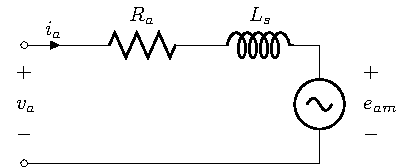
\includegraphics{figSynchronousMotorModel}
\caption{معاصر موٹر کا مساوی دور یا ریاضی نمونہ۔}
\label{شکل_معاصر_موٹر_کا_مساوی_دور}
\end{figure}
اگر موٹر کی بجائے ایک معاصر جنریٹر کی بات ہوتی تو یہ جنریٹر برقی دباؤ پیدا کرتا اور برقی رو اس جنریٹر کی مثبت سرے سے باہر کی جانب کو ہوتی۔ اس صورت میں ہمیں شکل \حوالہ{شکل_معاصر_موٹر_کا_مساوی_دور}  کی جگہ شکل \حوالہ{شکل_معاصر_جنریٹر_کا_مساوی_دور}  ملے گا۔اس شکل کی مساوات اسی شکل سے یوں حاصل ہوتی ہے۔
\begin{figure}
\centering
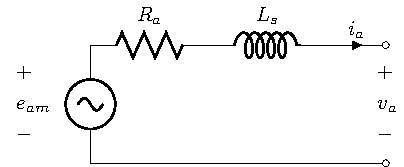
\includegraphics{figSynchronousGeneratorModel}
\caption{معاصر جنریٹر کا مساوی دور یا ریاضی نمونہ۔}
\label{شکل_معاصر_جنریٹر_کا_مساوی_دور}
\end{figure}

\begin{align}
e_{am}=i_a R_a+L_s \frac{\dif i_a}{\dif t}+v_a
\end{align}
یہاں یہ دھیان رہے کہ جنریٹر کے مساوی دور میں برقی رو کی مثبت سمت موٹر کے مساوی دور میں برقی رو کی مثبت سمت کے اُلٹ ہے۔اس کا مرحلی سمتیہ\فرہنگ{مرحلی سمتیہ} مساوات یوں لکھا جائے گا۔
\begin{align}\label{مساوات_معاصر_جنریٹر_دوری_سمتیہ_مساوات}
\hat{E}_{am}= \hat{I}_a R_a+j \hat{I}_a X_s +\hat{V}_a
\end{align}
اس مرحلی سمتیہ کے مساوات کو شکل \حوالہ{شکل_معاصر_جنریٹر_کے_سادہ_مساوی_دور}-الف میں دکھایا گیا ہے۔عام حالات میں \عددیء{X_s} کی مقدار  \عددیء{R_a} سے سو سے دو سو گنا زیادہ ہوتی ہے۔ 
\begin{figure}
\centering
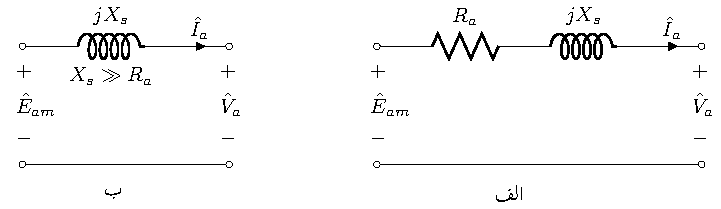
\includegraphics{figSynchronousGeneratorEquivalentCircuits}
\caption{معاصر جنریٹر کے مساوی دور۔}
\label{شکل_معاصر_جنریٹر_کے_سادہ_مساوی_دور}
\end{figure}

\ابتدا{مثال}
دو قطب \عددیء{50} ہرٹز کا ایک معاصر جنریٹر \عددیء{40} ایمپیئر میدانی برقی رو پر  \عددیء{2100} وولٹ یک مرحلہ موثر برقی دباؤ پیدا کرتی ہے۔اس مشین کی قوی اور میدانی لچھوں کے مابین مشترکہ امالہ حاصل کریں۔

	حل:
	مساوات \حوالہ{مساوات_معاصر_موثر_پیدا_دباؤ}  سے 
\begin{align}
L_{am}=\frac{\sqrt{2} E_{am}}{\omega I_m}=\frac{\sqrt{2}  \times 2100}{2 \times \pi \times 50 \times 40}=\SI{0.2363}{\henry}
\end{align}
\انتہا{مثال}
%
\حصہ{برقی طاقت کی منتقلی}
شکل \حوالہ{شکل_ٹرانسفارمر_سادہ_ماڈل} ٹرانسفارمر کا مساوی دور (ریاضی نمونہ) اور شکل \حوالہ{شکل_معاصر_جنریٹر_کے_سادہ_مساوی_دور} معاصر جنریٹر کا مساوی دور (ریاضی نمونہ) ہے۔ دونوں بالکل ایک طرح کے ہیں، لہٰذا مندرجہ ذیل بیان دونوں کے لئے درست ہو گا، اگرچہ یہاں ہمیں صرف معاصر آلوں سے دلچسپی ہے۔

معاصر آلوں میں معاصر متعاملہ لچھے کی مزاحمت سے بہت زیادہ ہوتا ہے لہٰذا اس کے مزاحمت کو نظرانداز کیا جا سکتا ۔ ایسا ہی شکل کے حصہ با میں کیا گیا ہے۔

شکل \حوالہ{شکل_معاصر_جنریٹر_کے_سادہ_مساوی_دور}-ب کو اگر ہم ایک لمحے کے لئے ایک سادہ برقی دور سمجھیں جس کے بائیں جانب \عددیء{\hat{E}_{am}} اور دائیں جانب \عددیء{\hat{V}_a} برقی دباؤ ہے جن کے مابین ایک متعاملہ \عددیء{j X_s} جڑا ہے۔ اس برقی دور میں برقی طاقت کے منتقلی کا حساب یوں ممکن ہے۔

 شکل \حوالہ{شکل_معاصر_جنریٹر_کے_سادہ_مساوی_دور}-ب کی مرحلی سمتیہ شکل \حوالہ{شکل_معاصر_جنریٹر_دوری_سمتیہ}  میں دی گئی ہے۔شکل \حوالہ{شکل_معاصر_جنریٹر_دوری_سمتیہ}-الف میں  برقی رو \عددیء{\hat{I}_a} برقی دباؤ \عددیء{\hat{V}_a} سے  \عددیء{\phi} زاویہ  پیچھے  ہے اور شکل \حوالہ{شکل_معاصر_جنریٹر_دوری_سمتیہ}-ب میں برقی رو \عددیء{\phi} زاویہ برقی دباؤ سے  آگے  ہے۔ چونکہ زاویہ اُفقی سمت سے گھڑی کی اُلٹی سمت ناپا جاتا ہے لہٰذا شکل-الف میں \عددیء{\phi} منفی زاویہ ہے اور \عددیء{\sigma} مثبت زاویہ ہے جبکہ شکل-ب میں دونوں زاویے مثبت ہیں۔
\begin{figure}
\centering
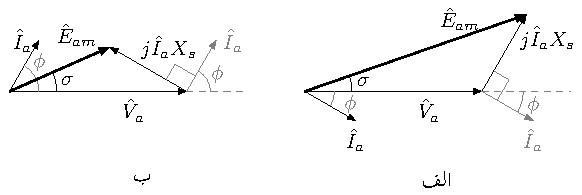
\includegraphics{figSynchronousGeneratorPhasorDiagram}
\caption{معاصر جنریٹر کا مرحلی سمتیہ۔}
\label{شکل_معاصر_جنریٹر_دوری_سمتیہ}
\end{figure}

دائیں جانب طاقت \عددیء{p_v} منتقل ہو رہی ہے جہاں
\begin{align}\label{مساوات_معاصر_طاقت_کی_منتقلی_الف}
p_v=V_a I_a \cos \phi
\end{align}
کے برابر ہے۔شکل \حوالہ{شکل_معاصر_جنریٹر_دوری_سمتیہ}-الف سے
\begin{gather}
\begin{aligned}
\hat{I}_a=I_a \phase{\phi_a}&=\frac{\hat{E}_{am}-\hat{V}_a}{j X_s}\\
&=\frac{E_{am} \phase{\sigma} -V_a \phase {0}}{X_s \phase{\frac{\pi}{2}}}\\
&=\frac{E_{am} \phase{\sigma-\pi/2} -V_a \phase {-\pi/2}}{X_s}
\end{aligned}
\end{gather}
لکھا جا سکتا ہے۔ایک مرحلی سمتیہ کے دو جزو ہوتے ہیں۔ اس کا حقیقی جزو اُفقی سمت میں بنایا جاتا ہے اور اس کا فرضی جزو حقیقی جزو کے عمود میں بنایا جاتا ہے۔شکل \حوالہ{شکل_معاصر_جنریٹر_دوری_سمتیہ} سے واضح ہے کہ اس مساوات کا حقیقی جزو  \عددیء{\hat{V}_a} کے ہم قدم ہے لہٰذا
\begin{gather}
\begin{aligned}
I_a \cos \phi_a&=\frac{E_{am}}{X_s} \cos \left(\sigma -\frac{\pi}{2} \right)-\frac{V_a}{X_s} \cos \left(-\frac{\pi}{2} \right)\\
&=\frac{E_{am}}{X_s} \sin \sigma
\end{aligned}
\end{gather}
اس مساوات اور مساوات \حوالہ{مساوات_معاصر_طاقت_کی_منتقلی_الف}  سے حاصل ہوتا ہے
\begin{align}\label{مساوات_معاصر_سائن_خصوصیات}
p_v=\frac{V_a E_{am}}{X_s} \sin \sigma
\end{align}
تین مرحلہ معاصر مشین کے لئے اس مساوات کو تین سے ضرب دیں یعنی
\begin{align}
p_v=\frac{3 V_a E_{am}}{X_s} \sin \sigma
\end{align}
یہ طاقت بالمقابل زاویہ\فرہنگ{طاقت بالمقابل زاویہ}\حاشیہب{power-angle law}\فرہنگ{power-angle law} کا قانون ہے۔اگر \عددیء{V_a} معین ہو تو جنریٹر \عددیء{E_{am}} یا \عددیء{\sigma} بڑھا کر طاقت بڑھا سکتا ہے۔\عددیء{E_{am}} گھومتے لچھے میں برقی رو بڑھا کر بڑھائی جاتی ہے۔البتہ یہ ایک حد تک کرنا ممکن ہے۔ لچھے کی مزاحمت میں برقی توانائی ضائع ہونے سے یہ گرم ہوتا ہے اور اس کی حرارت کو خطرناک حد تک پہنچنے نہیں دیا جا سکتا۔ دوسری جانب \عددیء{\sigma} کو نوے زاویہ تک بڑھایا جا سکتا ہے اور اس صورت میں جنریٹر زیادہ سے زیادہ طاقت مہیا کرے گا۔
\begin{align}\label{مساوات_معاصر_طاقت_انتہا}
p_{v,\textup{انتہا}}=\frac{3 V_a E_{am}}{X_s}
\end{align}
حقیقت میں جنریٹر کو اس طرح بنایا جاتا ہے کہ اس کی زیادہ سے زیادہ قابلِ استعمال طاقت نوے درجے سے کافی کم زاویہ پر ہو۔ نوے درجے پر جنریٹر کو قابو رکھنا مشکل ہو جاتا ہے۔
%
\begin{figure}
\centering
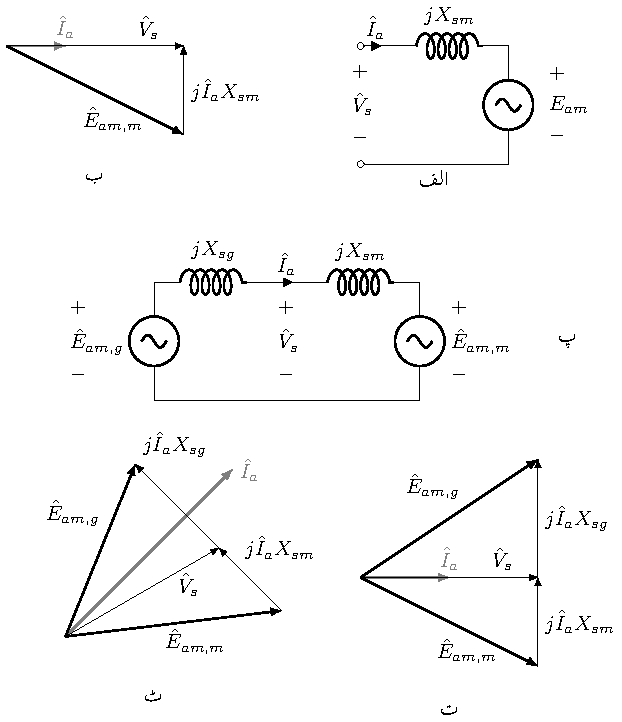
\includegraphics{figSynchronousGeneratorConnectedToMotor}
\caption{معاصر جنریٹر معاصر موٹر چلا رہی ہے۔}
\label{شکل_معاصر_جنریٹر_موٹر_چلاتا_ہوا}
5\end{figure}
\ابتدا{مثال}
ایک \عددیء{50} قطب ستارہ جڑی تین مرحلہ \عددیء{50} ہرٹز \عددیء{2300} وولٹ تار کی برقی دباؤ پر چلنے والی \عددیء{1800} کلو وولٹ-ایمپیئر کی معاصر مشین کی یک مرحلہ  معاصر امالہ \عددیء{2.1} اوہم ہے۔
\begin{itemize}
\item
مشین کے برقی سروں پر \عددیء{2300} وولٹ تار کی برقی دباؤ مہیا کرتے ہوئے اگر اس کی میدانی برقی رو اتنی رکھی جائے کہ پورے بوجھ پر مشین کا جزو طاقت ایک کے برابر ہو تو اس سے زیادہ سے زیادہ کتنی قوت مروڑ حاصل کی جا سکتی ہے۔
\item
اگر اسے  \عددیء{2}  قطب  \عددیء{3000} چکر فی منٹ تین مرحلہ ستارہ جڑی \عددیء{2300} وولٹ تار کی برقی دباؤ پیدا کرنے والی \عددیء{2200}  کلو وولٹ-ایمپیئر کی معاصر جنریٹر سے چلایا جائے جس کی یک مرحلہ معاصر امالہ \عددیء{2.3} اوہم ہو۔موٹر پر اس کا پورا برقی بوجھ لاد کر جنریٹر کو معاصر رفتار پر چلاتے ہوئے دونوں مشینوں کی میدانی برقی رو تبدیل کی جاتی ہے حتیٰ کہ موٹر ایک جزو طاقت پر چلنے لگے۔دونوں مشینوں کی میدانی برقی رو یہاں برقرار رکھ کر موٹر پر بوجھ آہستہ آہستہ بڑھائی جاتی ہے۔اس صورت میں موٹر سے زیادہ سے زیادہ کتنی قوت مروڑ  حاصل کی جا سکتی ہے اور اس کی سروں پر تار کی برقی دباؤ کتنی ہو گی۔ 
\end{itemize}

حل:
\begin{itemize}
\item
شکل \حوالہ{شکل_معاصر_جنریٹر_موٹر_چلاتا_ہوا}-الف اور \حوالہ{شکل_معاصر_جنریٹر_موٹر_چلاتا_ہوا}-ب سے رجوع کریں۔یک مرحلہ برقی دباؤ اور کُل برقی رو یہ ہیں
\begin{align*}
\frac{2300}{\sqrt{3}}=\SI{1327.9}{\volt}\\
\frac{1800000}{\sqrt{3} \times 2300}=\SI{451.84}{\ampere}
\end{align*}
لہٰذا
\begin{align*}
\hat{E}_{am,m}&=\hat{V}_a-j \hat{I}_a X_{s,m}\\
&=1327.9 \phase {0\degree} -j 451.84 \phase {0\degree} \times 2.1\\
&=1327.9-j 948.864\\
&=1632 \phase{-35.548\degree}
\end{align*}
ہے۔یوں مساوات \حوالہ{مساوات_معاصر_طاقت_انتہا}  سے ایک مرحلے کی زیادہ سے زیادہ برقی طاقت
\begin{align*}
p_{\textup{انتہا}}=\frac{1327.9 \times 1632}{2.1}=\SI{1031968}{\watt}
\end{align*}
ہے ۔یوں تین مرحلوں کی زیادہ سے زیادہ طاقت \عددیء{\num{3095904}} واٹ ہو گی۔\عددیء{50} ہرٹز اور \عددیء{50} قطب سے مشین کی معاصر میکانی رفتار مساوات
 \حوالہ{مساوات_گھومتے_مشین_برقی_میکانی_رفتار_تعلق}  کی مدد سے دو چکر فی سیکنڈ حاصل ہوتی ہے یعنی \عددیء{f_m=2}۔یوں مشین سے زیادہ سے زیادہ قوت مروڑ
\begin{align*}
T_{\textup{انتہا}}=\frac{p_{\textup{انتہا}}}{2 \pi f_m}=\frac{3095904}{2 \times \pi \times 2}=\SI{246364}{\newton \meter}
\end{align*}
حاصل ہو گی۔
%
\item
شکل \حوالہ{شکل_معاصر_جنریٹر_موٹر_چلاتا_ہوا}-پ سے رجوع کریں۔پہلی جزو کی طرح یہاں بھی موٹر کی برقی سروں پر تار کی برقی دباؤ  \عددیء{2300} وولٹ اور اس کی محرک برقی دباؤ \عددیء{1632} وولٹ ہے۔ جنریٹر کی محرک برقی دباؤ
\begin{align*}
\hat{E}_{am,g}&=\hat{V}_a+j  \hat{I}_a X_{s,g}\\
&=1327.9 \phase {0\degree} +j 451.84 \phase {0\degree} \times 2.3\\
&=1327.9+j 1039.233\\
&=1686 \phase{38.047\degree}
\end{align*}
ہے۔یہ صورت شکل \حوالہ{شکل_معاصر_جنریٹر_موٹر_چلاتا_ہوا}-ت میں دکھائی گئی ہے۔

معاصر موٹر اس وقت زیادہ سے زیادہ طاقت پیدا کرے گی جب  \عددیء{\hat{E}_{am,g}} اور \عددیء{\hat{E}_{am,m}} آپس میں \عددیء{90\degree} زاویہ پر ہوں۔ ایسا شکل \حوالہ{شکل_معاصر_جنریٹر_موٹر_چلاتا_ہوا}-ٹ میں دکھایا گیا ہے ۔

اب مساوات \حوالہ{مساوات_معاصر_طاقت_انتہا}  میں ایک معاصر امالہ کی جگہ سلسلہ وار جڑی موٹر اور جنریٹر کی امالہ ہیں اور دو برقی دباؤ اب موٹر اور جنریٹر کی محرک برقی دباؤ ہیں۔یوں موٹر کی یک مرحلہ  زیادہ سے زیادہ طاقت
\begin{align*}
p_{\textup{انتہا}}=\frac{1686 \times 1632}{2.3+2.1}=\SI{625352}{\watt}
\end{align*}	
حاصل ہوں گے۔تین مرحلوں سے یوں  \عددیء{\num{1876056 }} واٹ حاصل ہوں گے اور زیادہ سے زیادہ قوت مروڑ
\begin{align*}
T_{\textup{انتہا}}=\frac{1876056}{2 \times \pi \times 2}=\SI{149291}{\newton \meter}
\end{align*}
ہو گی۔
\end{itemize}
\انتہا{مثال}
%
\حصہ{یکساں حال، برقرار چالو مشین کے خصوصیات}
\جزوحصہ{معاصر جنریٹر: برقی بوجھ بالمقابل \عددیء{I_m} کے خطوط}
شکل \حوالہ{شکل_معاصر_جنریٹر_کے_سادہ_مساوی_دور}-ب کے لئے مرحلی سمتیوں کا مساوات یہ ہے
\begin{align}\label{مساوات_معاصر_دوری_جنریٹر_مساوات}
\hat{E}_{am}=\hat{V}_a+j \hat{I}_a X_s
\end{align}
اسے یوں لکھ سکتے ہیں
\begin{align}
E_{am}\phase{\sigma}=V_a \phase{0} +I_a X_s \phase{\frac{\pi}{2}+\phi}
\end{align}
اس مساوات کو مخلوط عدد\فرہنگ{مخلوط عدد}\حاشیہب{complex number} کے طور پر یوں لکھ سکتے ہیں۔
\begin{align*}
E_{am} \cos \sigma +j E_{am} \sin \sigma&=V_a \cos 0+j V_a \sin 0 + I_a X_s \cos \left(\frac{\pi}{2}+\phi \right)+j I_a X_s \sin \left(\frac{\pi}{2}+\phi \right)\\
&=E_{am,x}+j E_{am,y}
\end{align*}
اس مساوات سے \عددیء{\abs{\hat{E}_{am}}} یعنی \عددیء{E_{am}} کی مقدار یوں حاصل ہوتی ہے۔
\begin{gather}
\begin{aligned}
\abs{\hat{E}_{am}}=E_{am}&=\sqrt{E_{am,x}^2+E_{am,y}^2}\\
&=\sqrt{V_a^2+\left(I_a X_s\right)^2 +2 V_a I_a X_s \sin \phi}
\end{aligned}
\end{gather}
جنریٹر کے سروں پر معین \عددیء{V_a} رکھتے ہوئے مختلف \عددیء{\phi} کے لئے \عددیء{E_{am}} بالمقابل \عددیء{I_a} کے خط شکل \حوالہ{شکل_معاصر_بار_بالمقابل_میدانی_رو}  میں دکھائے گئے ہیں۔ چونکہ \عددیء{E_{am}}  اور  \عددیء{I_m} براہِ راست متناسب ہیں اور اسی طرح کسی ایک مخصوص جزو طاقت اور معین \عددیء{V_a} کے لئے جنریٹر کا طاقت \عددیء{I_a} کے  براہِ راست متناسب ہوتا ہے لہٰذا یہی گراف \عددیء{I_m} بالمقابل جنریٹر کے طاقت کو بھی ظاہر کرتا ہے۔
\begin{figure}
\centering
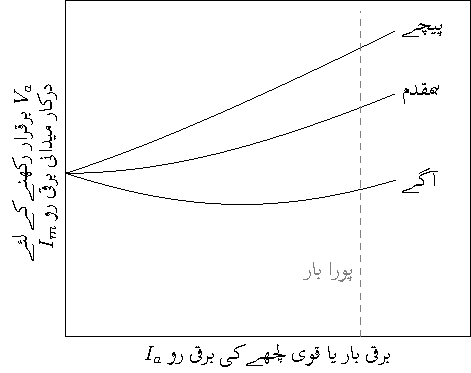
\includegraphics{figSynchronousCompoundingCurves}
\caption{جنریٹر: برقی بوجھ بالمقابل \عددیء{I_m} کے خط}
\label{شکل_معاصر_بار_بالمقابل_میدانی_رو}
\end{figure}
\جزوحصہ{معاصر موٹر:\عددیء{I_a}   بالمقابل \عددیء{I_m}  کے خط}
معاصر موٹر کا مساوی دور (ریاضی نمونہ) شکل \حوالہ{شکل_معاصر_موٹر_کا_مساوی_دور}  میں دکھایا گیا ہے اور اس کا مرحلی سمتیہ شکل  \حوالہ{شکل_معاصر_موٹر_کی_دوری_سمتیہ} میں دکھایا گیا ہے۔ اس میں مزاحمت نظرانداز کرنے سے اس کی مساوات یوں ہو گی۔
\begin{gather}
\begin{aligned}
\hat{V}_a&=\hat{E}_{am}+j \hat{I}_a X_s\\
V_a \phase{0}&=E_{am} \phase{\sigma} +j I_a \phase{\phi} X_s\\
&=E_{am} \phase{\sigma} +I_a X_s \phase{\frac{\pi}{2}+\phi}
\end{aligned}
\end{gather}
اس مساوات میں زاویے موٹر پر لاگو برقی دباؤ \عددیء{\hat{V}_a} کے حوالہ سے ہیں، یعنی \عددیء{\hat{V}_a}  کا زاویہ صفر لیا گیا ہے۔یاد رہے کہ زاویہ ناپنے کی مثبت سمت اُفقی لکیر سے گھڑی کی اُلٹی سمت ہے لہٰذا \اصطلاح{پیش} زاویہ\حاشیہب{leading angle} مثبت اور \اصطلاح{تاخیری} زاویہ\حاشیہب{lagging angle} منفی ہیں۔ اس مساوات سے امالی دباؤ \عددیء{E_{am}} کی مقدار یوں حاصل ہو گی۔
\begin{align*}
E_{am}\phase{\sigma}&=V_a \phase{0}-I_a X_s \phase{\frac{\pi}{2}+\phi}\\
&=V_a -I_a X_s  \cos \left( \frac{\pi}{2}+\phi\right)- j I_a X_s \sin \left(\frac{\pi}{2}+\phi \right)\\
&=V_a +I_a X_s \sin \phi-j I_a X_s \cos \phi
\end{align*}
لہٰذا
\begin{gather}
\begin{aligned}\label{مسوات_معاصر_دوری_مساوات}
\abs{E_{am}}&=\sqrt{\left(V_a +I_a X_s \sin \phi \right)^2+\left(I_a X_s \cos \phi \right)^2}\\
&=\sqrt{V_a^2+I_a^2 X_s^2+ 2 V_a I_a X_s \sin \phi}
\end{aligned}
\end{gather}
موٹر پر لاگو برقی دباؤ اور اس پر میکانی بوجھ کو \عددیء{0 \%}، \عددیء{25 \%} اور \عددیء{75 \%} پر رکھ کر اس مساوات کو شکل \حوالہ{شکل_معاصر_برقی_رو_بالمقابل_برقی_دباؤ}   میں  گراف کیا گیا ہے۔ یہ موٹر کے \عددیء{E_{am}} بالمقابل  \عددیء{I_a} خط ہیں۔ چونکہ امالی دباؤ \عددیء{I_m} کے براہِ راست متناسب ہے لہٰذا یہی موٹر کے \عددیء{I_m} بالمقابل \عددیء{I_a} خط بھی ہیں۔ان میں سے ہر خط ایک معین میکانی بوجھ \عددیء{p} کے لئے ہے جہاں
\begin{align}\label{مساوات_معاصر_طاقت_برابر_دباؤ_رو_جزو_طاقت}
p=V_a I_a \cos \phi
\end{align}
%
\begin{figure}
\centering
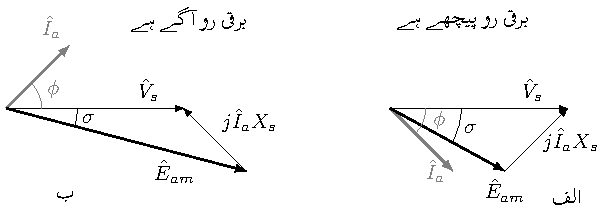
\includegraphics{figSynchronousMotorPhasorDiagram}
\caption{موٹر کا مرحلی سمتیہ۔}
\label{شکل_معاصر_موٹر_کی_دوری_سمتیہ}
5\end{figure}
%
اس مساوات سے واضح ہے کہ اگر \عددیء{p} اور \عددیء{V_a} معین ہوں تو جزو طاقت تبدیل کر کے \عددیء{I_a} تبدیل کیا جا سکتا ہے۔لہٰذا مساوت \حوالہ{مسوات_معاصر_دوری_مساوات}  کو مساوات \حوالہ{مساوات_معاصر_طاقت_برابر_دباؤ_رو_جزو_طاقت}  کی مدد سے گراف کیا جاتا ہے۔ یہ کچھ یوں کیا جاتا ہے۔معین \عددیء{V_a} اور \عددیء{p} کے لئے مختلف \عددیء{I_a} پر مساوات \حوالہ{مساوات_معاصر_طاقت_برابر_دباؤ_رو_جزو_طاقت}   سے \عددیء{\phi} حاصل کریں۔ ان \عددیء{I_a} اور \عددیء{\phi} کو مساوات  \حوالہ{مسوات_معاصر_دوری_مساوات} میں استعمال کر کے \عددیء{E_{am}} کا حساب لگائیں اور \عددیء{E_{am}} بالمقابل \عددیء{I_a} کا گراف بنائیں۔

موٹر کی ان خطوط سے واضح ہے کہ \عددیء{I_m} کو تبدیل کر کے موٹر کی جزو طاقت تبدیل کی جا سکتی ہے۔ لہٰذا موٹر کو \اصطلاح{پیش} زاویہ یا \اصطلاح{تاخیری} زاویہ  پر چلایا جا سکتا ہے۔ اگر اسے پیش زاویہ پر رکھا جائے تو یہ ایک کپیسٹر\فرہنگ{کپیسٹر}\حاشیہب{capacitor}  کے طور پر استعمال ہو سکتا ہے اگرچہ ایسا کیا نہیں جاتا چونکہ کپیسٹر از خود  زیادہ سستا ہوتا ہے۔ 
\begin{figure}
\centering
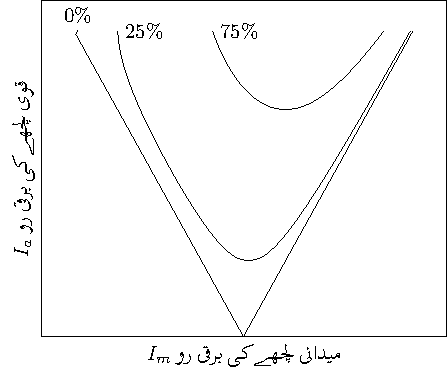
\includegraphics{figSynchronousVcurves}
\caption{موٹر:$I_{m}$ بالمقابل $I_a$ کے خط}
\label{شکل_معاصر_برقی_رو_بالمقابل_برقی_دباؤ}
\end{figure}
\حصہ{کھلے دور  اور کسرِ دور  معائنہ }
معاصر مشین کے مساوی دور بنانے کے لئے اس کے جزو معلوم کرنا لازم ہے۔یہ دو قسم کے معائنوں سے کیا جاتا ہے۔ انہیں کھلے دور معائنہ اور کسرِ دور معائنہ کہتے ہیں۔ان معائنوں سے قالب کے سیراب ہونے کے اثرات بھی سامنے آتے ہیں۔ہم نے ٹرانسفارمر کے لئے بھی اسی قسم کے معائنے کیے تھے۔وہاں ہم نے دیکھا تھا کہ کُھلے دور معائنہ اس برقی دباؤ پر کیا جاتا ہے جتنے کے لئے مشین بنائی\حاشیہب{design}\فرہنگ{design} گئی ہو جبکہ کسرِ دور معائنہ اس برقی رو پر کیا جاتا ہے جتنے کے لئے مشین بنائی گئی ہو۔یہاں بھی ایسا ہی کیا جائے گا۔ 

\جزوحصہ{کُھلے دور معائنہ}
معاصر مشین کے برقی سرے کُھلے رکھ کر اور اسے معاصر رفتار پر گُھماتے ہوئے مختلف \عددیء{I_m} پر  مشین کے سروں پر پیدا برقی دباؤ \عددیء{V_a} ناپی جاتی ہے ۔ان دو کا گراف شکل \حوالہ{شکل_معاصر_کھلے_دور_خط}-الف میں دکھایا گیا ہے۔ یہ خط مشین کے کُھلے دور خاصیت ظاہر کرتا ہے۔ یہی خط مشین بنانے والے بھی مہیا کر سکتے ہیں۔

اس کتاب کے حصہ \حوالہ{حصہ_مقناطیسی_دور_مقناطیسی_مادہ_کے_خصوصیات} میں بتلایا گیا تھا کہ قالب پر لاگو مقناطیسی دباؤ اگر بڑھایا جائے تو اس میں مقناطیسی بہاو بڑھتی ہے البتہ جلد ہی قالب سیراب ہونے لگتا ہے۔اس کا اثر شکل-الف میں خط کے جھکنے سے واضح ہے۔اگر قالب سیراب نہ ہوتا تو یہ خط شکل میں دیئے سیدھی لکیر کی پیروی کرتا۔شکل میں مشین کا پورا برقی دباؤ اور اس  پر درکار برقی رو \عددیء{I_{m0}} دکھلایا گیا ہے۔
\begin{figure}
\centering
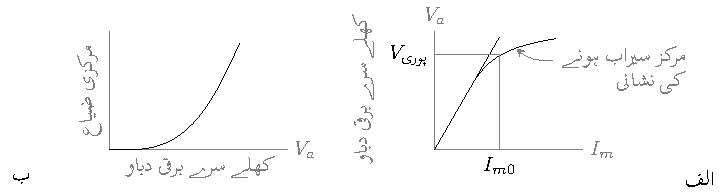
\includegraphics{figSynchronousOpenCircuitCharacteristic}
\caption{کُھلے دور خط اور قالبی ضیاع۔}
\label{شکل_معاصر_کھلے_دور_خط}
\end{figure}

یہ معائنہ کرتے وقت اگر دھرے پر میکانی طاقت \عددیء{p_1} ناپی جائے تو یہ بے بوجھ مشین کی طاقت کے ضیاع کے برابر ہو گی۔ اس کا بیشتر حصہ رگڑ کی وجہ سے، کچھ حصہ قالب میں ضیاع کی وجہ سے اور کچھ گھومتے لچھے میں ضیاع کی وجہ سے ہو گا۔یاد رہے کہ عموماً گھومتے لچھے کو یک سمتی جنریٹر سے برقی توانائی دی جاتی ہے اور یہ جنریٹر بھی مشین کے دھرے پر ہی نسب ہوتا ہے لہٰذا اسے طاقت محرک\حاشیہد{گھومتے لچھے کو توانائی یک سمتی جنریٹر سے آتی ہے اور اس جنریٹر کو دھرے سے آتی ہے۔} سے ہی ملتی ہے۔ بے بوجھ مشین اور بوجھ بردار مشین دونوں کا رگڑ سے طاقت کے ضیاع کو یکساں سمجھا جاتا ہے چونکہ رگڑ سے طاقت کے ضیاع کا مشین پر لدے بوجھ سے کوئی خاص تعلق نہیں۔ اب اگر یہی معائنہ دوبارہ کیا جائے لیکن اس مرتبہ \عددیء{I_m} بھی صفر رکھا جائے تو اس مرتبہ ناپا گیا طاقت \عددیء{p_2} صرف رگڑ کی وجہ سے طاقت کے ضیاع کے برابر ہو گا۔ان دو ناپے گئے طاقت کا فرق یعنی \عددیء{(p_1-p_2)} قالب میں طاقت کے ضیاع  اور گھومتے لچھے میں برقی ضیاع کے برابر ہو گا۔گھومتے لچھے میں برقی ضیاع بہت کم ہوتا ہے اور اس کو عموماً قالب کے ضیاع کا حصہ ہی تصور کیا جاتا ہے۔ اس طرح ناپے گئے قالبی ضیاع کا ایک خط شکل  \حوالہ{شکل_معاصر_کھلے_دور_خط}-ب میں دیا گیا ہے۔

\جزوحصہ{کسرِ دور معائنہ}
معاصر مشین کو معاصر رفتار پر جنریٹر کے طور چلاتے ہوئے اس کے ساکن لچھے کے سرے کسرِ دور کر کے مختلف \عددیء{I_m} پر کسرِ دور برقی رو \عددیء{I_a} ناپی جاتی ہے۔ ان دو کا گراف شکل \حوالہ{شکل_معاصر_کسر_دور_اور_کھلے_دور_خط}-الف میں دکھایا گیا ہے۔یہ خط کسرِ دور مشین کی خاصیت دکھلاتا ہے۔  یہ معائنہ کرتے وقت یہ دھیان رکھنا بہت اہم ہے کہ \عددیء{I_a} کی مقدار کہیں خطرناک حد تک نہ بڑھ جائے لہٰذا اسے جنریٹر کے پورے برقی بوجھ\فرہنگ{پورا بوجھ}\حاشیہب{full load} پر \عددیء{I_{a}} کی مقدار  یا اس کی دگنی مقدار سے کم رکھنا ضروری ہے ورنہ مشین گرم ہو کر تباہ ہو سکتی ہے۔کسرِ دور مشین میں، ڈیزائن کردہ برقی دباؤ کے، صرف دس سے پندرہ فی صد برقی دباؤ پر ہی اس میں سو فی صد برقی رو شروع ہو جاتی ہے۔ اتنا کم برقی دباؤ حاصل کرنے کے لئے خلائی درز میں اسی تناسب سے  کم مقناطیسی بہاو درکار ہوتا ہے۔ 
\begin{figure}
\centering
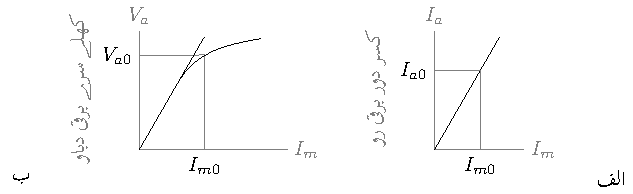
\includegraphics{figSynchronousShortCircuitCharacteristic}
\caption{کسرِ دور خط اور کھلے دور خط۔}
\label{شکل_معاصر_کسر_دور_اور_کھلے_دور_خط}
\end{figure}

شکل \حوالہ{شکل_معاصر_جنریٹر_کے_سادہ_مساوی_دور}  میں جنریٹر کے مساوی برقی دور دکھائے گئے ہیں۔ اسے شکل \حوالہ{شکل_معاصر_امالہ_معاصر}  میں کسرِ دور کر کے دکھایا گیا ہے۔یہاں سے واضح ہے کہ
\begin{align}
\hat{E}_{am}=\hat{I}_a R_a+j \hat{I}_a X_s
\end{align}
\عددیء{R_a} کو نظر انداز کر کے اس مساوات سے معاصر امالہ یوں حاصل کیا جا سکتا ہے۔
\begin{align}
X_s=\frac{\abs{\hat{E}_{am}}}{\abs{\hat{I}_a}}=\frac{E_{am}}{I_a}
\end{align}
%
\begin{figure}
\centering
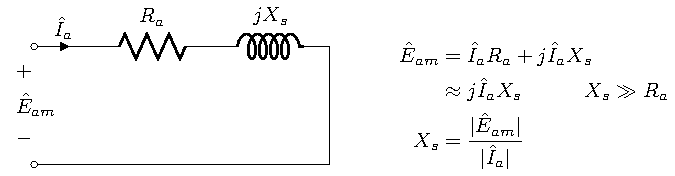
\includegraphics{figSynchronousReactanceSynchronous}
\caption{معاصر امالہ۔}
\label{شکل_معاصر_امالہ_معاصر}
\end{figure}
اس مساوات میں \عددیء{\hat{I}_a} کسرِ دور مشین کی برقی رو اور \عددیء{\hat{E}_{am}} اس کی اسی حال میں ایک دور کی امالہ برقی دباؤ ہے۔ کھلے دور مشین میں \عددیء{\hat{I}_a} صفر ہوتا ہے ۔مساوات \حوالہ{مساوات_معاصر_دوری_جنریٹر_مساوات} سے واضح ہے کہ اگر \عددیء{\hat{I}_a} صفر ہو تو \عددیء{\hat{E}_{am}}  اور \عددیء{\hat{V}_a} برابر ہوں گے۔ لہٰذا ہم کسی معین \عددیء{I_{m0}} پر شکل \حوالہ{شکل_معاصر_کسر_دور_اور_کھلے_دور_خط}-الف سے  \عددیء{I_{a0}} اور شکل \حوالہ{شکل_معاصر_کسر_دور_اور_کھلے_دور_خط}-ب سے \عددیء{V_{a0}} معلوم کرتے ہیں اور ان سے \عددیء{X_s} کا حساب لگاتے ہیں، یعنی
\begin{align}
X_s=\frac{V_{a0}}{I_{a0}}
\end{align}
معاصر امالہ عموماً مشین کے پورے برقی دباؤ پر معلوم کی جاتی ہے تا کہ قالب سیراب ہونے کے اثر کو بھی شامل کیا جائے۔شکل میں ایسا ہی کیا گیا ہے۔

معاصر امالہ مشین کو ستارہ نما تصور کر کے اس کا یک مرحلہ \عددیء{X_s} حاصل کیا جاتا ہے۔لہٰذا اگر معائنہ کرتے وقت مشین کی تار برقی دباؤ\حاشیہب{line voltage} ناپے گئے ہوں تو انہیں \عددیء{\sqrt{3}} سے تقسیم کر کے مشین کے یک مرحلہ برقی دباؤ حاصل کر کے مساوات میں استعمال کریں، یعنی
\begin{align}
V_{\textup{یکمرحلہ}}=\frac{V_{\textup{تار}}}{\sqrt{3}}
\end{align}
%
\ابتدا{مثال}
ایک  \عددیء{75}  کلو وولٹ-ایمپیئر ستارہ جڑی  \عددیء{415} وولٹ پر چلنے والی تین مرحلہ معاصر مشین کے کھلے دور اور کسرِ دور معائنے کئے گئے۔حاصل نتائج یہ ہیں۔
\begin{itemize}
\item
کھلے دور معائنہ:\عددیء{V_{\textup{تار}}=\SI{415}{\volt}} اور \عددیء{I_m=\SI{3.2}{\ampere}} ہیں۔
\item
کسر دور معائنہ:
جب قوی لچھے کی برقی رو \عددیء{\SI{104}{\ampere}} تھی تب میدانی لچھے کی برقی رو \عددیء{\SI{2.48}{\ampere}} تھی اور جب  قوی لچھے کی برقی رو \عددیء{\SI{126}{\ampere}} تھی تب میدانی لچھے کی برقی رو \عددیء{\SI{3.2}{\ampere}} تھی۔
\end{itemize}
اس مشین کی معاصر امالہ حاصل کریں۔

حل: یک مرحلہ برقی دباؤ
\begin{align*}
V_{\textup{یکمرحلہ}}=\frac{V_{\textup{تار}}}{\sqrt{3}}=\frac{415}{\sqrt{3}}=\SI{239.6}{\volt}
\end{align*}
ہے۔یہ کھلے دور برقی دباؤ  \عددیء{3.2}  ایمپیئر میدانی برقی رو پر حاصل ہوتی ہے۔ اتنی میدانی برقی رو پر کسرِ دور برقی رو  \عددیء{126} ایمپیئر ہیں لہٰذا یک مرحلہ معاصر امالہ 
\begin{align*}
X_s=\frac{239.6}{126}=\SI{1.901}{\ohm}
\end{align*}
  ہو گی۔
\انتہا{مثال}
%
کسرِ دور معائنہ کرتے وقت اگر دھرے پر لاگو میکانی طاقت \عددیء{p_3} ناپی جائے تو یہ کسرِ دور مشین کی کُل ضیاع ہو گی۔\عددیء{p_3} ناپتے وقت کسرِ دور برقی رو \عددیء{I_{a,3}} بھی ناپ لیں۔اس کا کچھ حصہ قالب کی برقی ضیاع، کچھ دونوں لچھوں میں برقی ضیاع اور کچھ رگڑ سے میکانی ضیاع سے ہے۔اب اگر اس سے پچھلے معائنہ میں ناپی گئی رگڑ کی ضیاع \عددیء{p_2} منفی کی جائے تو ہمیں لچھوں کی ضیاع اور قالب کی ضیاع ملتا ہے۔ جیسا اُوپر عرض کیا گیا کہ کسرِ دور مشین میں پورا برقی رو،  پورے برقی دباؤ کے صرف دس تا بیس فی صد پر حاصل ہو جاتا ہے اور اتنا کم برقی دباؤ حاصل کرنے کے لئے درکار مقناطیسی بہاو اتنا ہی کم ہوتا ہے۔ اتنے کم مقناطیسی بہاو پر قالب میں ضیاع کو نظر انداز کیا جا سکتا ہے۔ اسی طرح کسی بھی کسرِ دور معاصر مشین کے گھومتے لچھے میں برقی ضیاع ساکن لچھے میں برقی ضیاع سے بہت کم ہوتا ہے اور اسے بھی نظرانداز کیا جا سکتا ہے۔لہٰذا \عددیء{(p_3-p_2)} کو ساکن لچھے میں برقی ضیاع کے برابر لیا جاتا ہے۔شکل \حوالہ{شکل_معاصر_کسر_دور_ضیاع}  میں ایک ایسا ہی خط دکھایا گیا ہے۔لہٰذا
\begin{align*}
p_3-p_2=I_{a,3}^2 R_a
\end{align*}
اس مساوات سے معاصر مشین کی مساوی مزاحمت یوں حاصل ہوتی ہے۔
\begin{align}
R_a=\frac{p_3-p_2}{I_{a,3}^2}
\end{align}
%
\begin{figure}
\centering
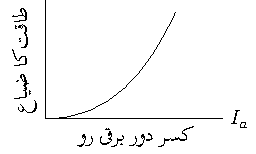
\includegraphics{figSynchronousShortCircuitedLoss}
\caption{کسرِ دور معاصر مشین میں طاقت کا ضیاع۔}
\label{شکل_معاصر_کسر_دور_ضیاع}
\end{figure}
\ابتدا{مثال}
ایک  \عددیء{75} کلو وولٹ-ایمپیئر  \عددیء{415} وولٹ پر چلنے والی تین مرحلہ معاصر مشین کے پورے برقی رو پر  کُل کسرِ دور طاقت کا ضیاع  \عددیء{2.2} کلو واٹ ہے۔ اس مشین کی یک مرحلہ موثر مزاحمت حاصل کریں۔

حل:یک مرحلہ ضیاع  \عددیء{\tfrac{2200}{3}=\SI{733.33}{\watt}}  ہے ۔مشین کے پوری برقی رو
\begin{align*}
\frac{75000}{\sqrt{3} V_{\textup{تار}}}=\SI{104.34}{\ampere}
\end{align*}
ہے۔لہٰذا
\begin{align*}
R_a=\frac{733.33}{104.34^2}=\SI{0.067}{\ohm}
\end{align*}
ہے۔
\انتہا{مثال}
%
\ابتدا{مثال}
شکل \حوالہ{شکل_معاصر_کھلے_دور_بریلووین_خط}  میں \عددیء{500} وولٹ، \عددیء{50} ہرٹز، \عددیء{4} قطب ستارہ جڑی معاصر جنریٹر کا کھلے دور خط دکھایا گیا ہے۔اس جنریٹر کا معاصر امالہ \عددیء{0.1} اوہم اور قوی لچھے کی مزاحمت \عددیء{0.01} اوہم ہے۔پورے برقی بوجھ پر جنریٹر \عددیء{0.92} تاخیری جزو طاقت\حاشیہب{lagging power factor} پر \عددیء{1000} ایمپیئر فراہم کرتا ہے۔پورے بوجھ پر رگڑ کے ضیاع اور لچھے کی مزاحمت میں ضیاع کا مجموعہ \عددیء{30} کلو واٹ جبکہ قالب کی ضیاع \عددیء{25} کلو واٹ ہے۔
\begin{itemize}
\item
جنریٹر کی رفتار معلوم کریں۔
\item
بے بوجھ جنریٹر کی سروں پر \عددیء{500} وولٹ برقی دباؤ کتنی میدانی برقی رو پر حاصل ہو گی۔
\item
اگر جنریٹر پر  \عددیء{0.92} تاخیری جزو طاقت، \عددیء{1000} ایمپیئر کا برقی بوجھ لادا جائے تو جنریٹر کے برقی سروں پر \عددیء{500} وولٹ برقرار رکھنے کے لئے کتنی میدانی برقی رو درکار ہو گی۔
\item
جنریٹر پورے بوجھ پر کتنی طاقت فراہم کر رہا ہے جبکہ اس کو محرک کتنی میکانی طاقت فراہم کر رہا ہے۔ان دو سے جنریٹر کی فی صد \اصطلاح{کارگزاری}\فرہنگ{کارگزاری}\حاشیہب{efficiency} حاصل کریں۔
\item
اگر جنریٹر سے یک دم برقی بوجھ ہٹایا جائے تو اس لمحہ اس کے برقی سروں پر کتنا برقی دباؤ ہو گا۔
\item
اگر جنریٹر پر \عددیء{1000} ایمپیئر  \عددیء{0.92}  پیش جزو طاقت والا بوجھ لادا جائے تو جنریٹر کے برقی سروں پر \عددیء{500} وولٹ برقرار رکھنے کے لئے کتنی میدانی برقی رو درکار ہو گی۔
\item
ان دو \عددیء{1000} ایمپیئر تاخیری جزو طاقت اور پیش جزو طاقت بوجھوں میں کونسی بوجھ زیادہ میدانی برقی رو پر حاصل ہوتی ہے۔جنریٹر کس بوجھ سے زیادہ گرم ہو گا۔
\end{itemize}
%
\begin{figure}
\centering
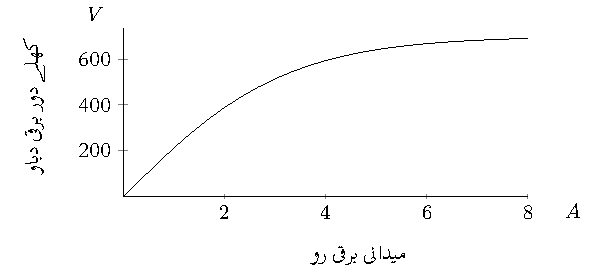
\includegraphics{figSynchronousOpenCircuitCharacteristicsBrillouinFunction}
\caption{کھلے دور خط۔}
\label{شکل_معاصر_کھلے_دور_بریلووین_خط}
\end{figure}
حل:
\begin{itemize}
\item
\عددیء{f_e=\tfrac{P}{2} f_m} سے \عددیء{f_m=\tfrac{2}{4} \times 50=25} چکر فی سیکنڈ یا \عددیء{25 \times 60=1500} چکر فی منٹ ہے۔
\item
شکل \حوالہ{شکل_معاصر_کھلے_دور_بریلووین_خط}  سے  \عددیء{500}  وولٹ کے لئے درکار میدانی برقی رو تقریباً \عددیء{2.86} ایمپیئر ہے۔
\item
ستارہ برقی دباو کے تعلق \عددیء{V_{\textup{تار}}=\sqrt{3} V_{\textup{یکمرحلہ}}} سے \عددیء{V_{\textup{یکمرحلہ}}=\tfrac{500}{\sqrt{3}}=289}  وولٹ حاصل ہوتا ہے۔ستارہ جوڑ میں یک مرحلہ برقی رو اور تار برقی رو برابر ہوتے ہیں۔جزو طاقت ستارہ یک مرحلہ برقی دباو کے نسبت سے بیان کیا جاتا ہے۔چونکہ \عددیء{\cos^{-1} 0.92=23.07\degree} ہے لہٰذا اگر برقی سروں پر دباو \عددیء{289 \phase {0 \degree}} لکھا جائے تو تاخیری دوری برقی رو \عددیء{1000\phase {-23.07 \degree}}  لکھی جائے گی۔یوں شکل \حوالہ{شکل_معاصر_جنریٹر_کا_مساوی_دور} یا مساوات \حوالہ{مساوات_معاصر_جنریٹر_دوری_سمتیہ_مساوات} سے اندرونی پیدا یک مرحلہ برقی دباو

\begin{align*}
\hat{E}_a&=\hat{V}_{a}+\hat{I}_a \left(R_a+j X_s \right)\\
&= 289\phase{0 \degree}+1000 \phase {-23.07 \degree} ( 0.01 +j 0.1)\\
&=349\phase{14.6 \degree}
\end{align*}
ہو گا جس سے اندرونی پیدا تار برقی دباو \عددیء{\sqrt{3} \times 349=604} وولٹ حاصل ہوتا ہے۔شکل \حوالہ{شکل_معاصر_کھلے_دور_بریلووین_خط} سے اتنی دباو کے لئے  \عددیء{\SI{4.1}{\ampere}} میدانی برقی رو درکار ہے۔
\item
جنریٹر اس صورت میں
\begin{align*}
p&=\sqrt{3} \hat{V}_{a} \cdot \hat{I}_a\\
&=\sqrt{3} \times 500 \times 1000 \times 0.92\\
&=\SI{796743}{\watt}
\end{align*}
فراہم کر رہا ہے جبکہ محرک 
\begin{align*}
p_m&=796.743+30+25=\SI{851.74}{\kilo \watt}
\end{align*}
فراہم کر رہا ہے لہٰذا اس جنریٹر کی کارگزاری \عددیء{\eta = \tfrac{796.743}{851.74} \times 100=93.54 \%} ہے۔
\item
اگر جنریٹر سے یک دم برقی بوجھ ہٹایا جائے تو اس لمحہ اس کے برقی سروں پر \عددیء{604}  وولٹ برقی دباو ہو گا۔
\item
پیش جزو طاقت کی صورت میں
\begin{align*}
\hat{E}_a&=\hat{V}_{a}+\hat{I}_a \left(R_a+j X_s \right)\\
&= 289\phase{0 \degree}+1000 \phase {23.07 \degree} ( 0.01 +j 0.1)\\
&=276\phase{20.32 \degree}
\end{align*}
درکار ہو گی جس سے اندرونی پیدا تار برقی دباو \عددیء{\sqrt{3} \times 276=478} وولٹ حاصل ہوتا ہے۔شکل \حوالہ{شکل_معاصر_کھلے_دور_بریلووین_خط} سے اتنی دباو کے لئے  \عددیء{\SI{2.7}{\ampere}} میدانی برقی رو درکار ہے۔
\item
تاخیری جزو طاقت کے بوجھ پر جنریٹر کو زیادہ میدانی برقی رو درکار ہے۔میدانی لچھے کی مزاحمت میں اس کی وجہ سے زیادہ برقی طاقت ضائع ہو گی اور جنریٹر یوں زیادہ گرم ہو گا۔
\end{itemize}
\انتہا{مثال}
%
\ابتدا{مثال}
ایک \عددیء{415} وولٹ، \عددیء{40} کلو وولٹ-ایمپیئر ستارہ جڑی \عددیء{0.8} جزو طاقت، \عددیء{50} ہرٹز پر چلنی والی معاصر موٹر کا معاصر امالہ \عددیء{2.2} اوہم ہے جبکہ اس کی مزاحمت قابل نظرانداز ہے۔اس کی رگڑ اور لچھوں کی مزاحمت میں طاقت کا ضیاع ایک کلو واٹ جبکہ قالبی ضیاع \عددیء{800} واٹ ہے۔یہ موٹر \عددیء{12.2}  کلوواٹ میکانی بوجھ سے لدی ہے اور یہ \عددیء{0.8}  پیش جزو طاقت   پر چل رہی ہے۔یاد رہے کہ معاصر امالہ مشین کو ستارہ نما تصور کرتے ہوئے حاصل کی جاتی ہے۔ 
\begin{itemize}
\item
اس کی مرحلی سمتیہ بنائیں۔تار کی برقی رو \عددیء{\hat{I}_t} اور قوی لچھے کی برقی رو  \عددیء{\hat{I}_a} حاصل کریں۔موٹر کی اندرونی ہیجانی برقی دباؤ \عددیء{\hat{E}_a} حاصل کریں۔
\item
میدانی برقی رو کو بغیر تبدیل کئے  میکانی بوجھ آہستہ آہستہ بڑھا کر دگنی کی جاتی ہے۔اس صورت میں موٹر کی ردِ عمل مرحلی سمتیہ سے واضح کریں ۔
\item
اس دگنی میکانی بوجھ پر قوی لچھے  کی برقی رو،  تار کی برقی رو  اور موٹر کی اندرونی ہیجانی برقی دباؤ حاصل کریں۔موٹر کی جزو طاقت بھی حاصل کریں۔
\end{itemize}

حل:
\begin{itemize}
\item
ستارہ جڑی موٹر کے سروں پر یک مرحلہ برقی دباو \عددیء{\tfrac{415}{\sqrt{3}}=\SI{239.6}{\volt}}  ہو گا جسے صفر زاویہ پر تصور کرتے ہوئے برقی رو کا زاویہ بیان کیا جاتا ہے۔یوں \عددیء{\hat{V}_{sa}=239.6\phase {0\degree}} لکھا جائے گا۔جزو طاقت \عددیء{0.8} زاویہ  \عددیء{36.87\degree} کو ظاہر کرتا ہے۔ یوں تار کی برقی رو کا \اصطلاح{پیش} زاویہ یہی ہو گا۔موٹر کو مہیا برقی طاقت اس کی میکانی طاقت اور طاقت کے ضیاع کے برابر ہو گی یعنی
\begin{align*}
\SI{12200}{\watt}+\SI{1000}{\watt}+\SI{800}{\watt}=\SI{14000}{\watt}
\end{align*}
جس  کے لئے درکار تار کی برقی رو 
\begin{align*}
I_t&=\frac{p}{\sqrt{3} V_{t} \cos \theta}\\
&=\frac{\num{14000}}{\sqrt{3} \times 415 \times 0.8}\\
&=\SI{24.346}{\ampere}
\end{align*}
ہو گی۔ستارہ جڑی موٹر کے قوی لچھے کی برقی رو تار کے برقی رو کے برابر ہو گی۔یوں برقی رو کا زاویہ شامل کرتے ہوئے اسے 
\begin{align*}
\hat{I}_a=\hat{I}_t=24.346 \phase {36.87 \degree}
\end{align*}
لکھا جا سکتا ہے۔

موٹر کا اندرونی یک مرحلہ ہیجانی برقی دباؤ موٹر کی مساوی دور شکل \حوالہ{شکل_معاصر_موٹر_کا_مساوی_دور}  کی مدد سے
\begin{align*}
\hat{E}_a&=\hat{V}_{a,s}- j X_s \hat{I}_a\\
&=239.6 \phase{0\degree}-j 2.2 \times 24.346 \phase{36.87\degree}\\
&=276 \phase{-8.96\degree}
\end{align*}
ہو گی۔یہ تمام صورت حال شکل \حوالہ{شکل_معاصر_بار_بردار_جنریٹر_مثال}  میں مرحلی سمتیات کی مدد سے دکھایا گیا ہے۔
\begin{figure}
\centering
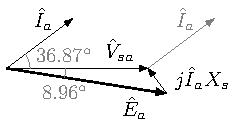
\includegraphics{figSynchronousLoadedGeneratorExample}
\caption{بوجھ بردار معاصر موٹر۔}
\label{شکل_معاصر_بار_بردار_جنریٹر_مثال}
\end{figure}
%
\item
میکانی بوجھ بڑھنے سے موٹر کو زیادہ برقی طاقت درکار ہو گی۔ یہ اس صورت ممکن ہو گا جب موٹر کے قوی لچھے کی برقی رو بڑھ سکے۔میدانی برقی رو معین ہونے کی وجہ سے موٹر کی اندرونی ہیجانی برقی دباؤ \عددیء{\hat{E}_a} کی مقدار تبدیل نہیں ہو سکتی البتہ اس کا زاویہ تبدیل ہو سکتا ہے۔موٹر  \عددیء{\hat{E}_a}  کی مقدار تبدیل کئے بغیر  برقی سروں پر لاگو برقی دباؤ  \عددیء{\hat{V}_a}  اور \عددیء{\hat{E}_a}  کے مابین زاویہ بڑھا کر قوی لچھے کی برقی رو اور یوں حاصل برقی طاقت بڑھائے گا۔ایسا شکل \حوالہ{شکل_معاصر_بار_بڑھانے_کا_اثر}  میں دکھایا گیا ہے۔شکل میں \عددیء{\hat{E}_a} مرحلی سمتیہ کی نوک نقطہ دار گول دائرہ پر رہتی ہے۔یوں اس کا طول تبدیل نہیں ہوتا۔زاویہ بڑھنے سے \عددیء{\abs{j\hat{I}_a X_s}} بڑھتا ہے۔چونکہ \عددیء{X_s} نہیں بڑھ رہا لہٰذا درحقیقت قوی لچھے کی برقی رو بڑھ گئی ہے۔زیادہ بوجھ کے متغیرات کو ہلکی سیاہی میں دکھایا گیا ہے۔
\begin{figure}
\centering
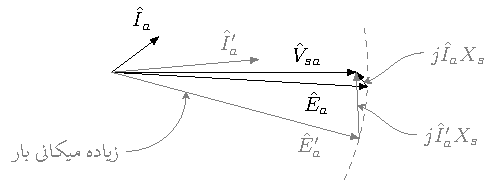
\includegraphics{figSynchronousLoadedGeneratorIncreasingLoad}
\caption{بوجھ بڑھنے کا اثر۔}
\label{شکل_معاصر_بار_بڑھانے_کا_اثر}
\end{figure}
%
\item
دگنی میکانی بوجھ پر موٹر کو کُل \عددیء{24400+800+1000=26200}  واٹ یا \عددیء{26.2}  کلو واٹ برقی طاقت درکار ہے۔مساوات \حوالہ{مساوات_معاصر_سائن_خصوصیات}  کی مدد سے
\begin{align*}
\sigma&=\sin^{-1} \left(\frac{p X_s}{3 V_a E_a} \right)=\sin^{-1} \left(\frac{26200 \times 2.2}{3\times 239.6 \times 276} \right)=16.89\degree
\end{align*}
یوں موٹر کی اندرونی ہیجانی برقی دباؤ \عددیء{276 \phase{-16.89\degree}} ہو گی اور قوی لچھے کی برقی رو
\begin{align*}
\hat{I}_a&=\frac{\hat{V}_a-\hat{E}_a}{j X_s}\\
&=\frac{239\phase{0\degree}-276\phase{-16.89\degree}}{j 2.2}\\
&=38\phase{17.4\degree}
\end{align*}
ہو گی۔ستارہ جوڑ کی وجہ سے \عددیء{\hat{I}_t} بھی اتنا ہی ہو گا۔پیش جزو طاقت \عددیء{\cos 17.4 \degree=0.954} ہے۔
\end{itemize}
\انتہا{مثال}
